%%%%%%%%%%%%%%%%%%%%%%%%%%%%%%%%
% This file is loaded as Section 4 (empirical) in the new structure.
% Filename retained for git history continuity.
%%%%%%%%%%%%%%%%%%%%%%%%%%%%%%%%

\section{실험적 확인}\label{sec:experimental_analysis}

\S\ref{sec:why_rsp_works}는 세 가지 분리된 메커니즘을 예측한다. RSP는 (i) 출력 분포를 평탄화·재배열해 \emph{token-level} branching을 열고, (ii) 그 branching이 디코딩 동안 의미적으로 다른 \emph{trajectory-level} 궤적으로 propagate되며, (iii) rollout 사이의 독립 재추첨이 그 분기들을 $N$번에 걸쳐 \emph{outcome-level} Pass@$N$으로 누적시킨다. 이 세 예측을 같은 순서로 검증한다. \S\ref{sec:performance}는 RSP가 baseline 정확도를 보존하거나 회복하는 setting을 짚어 메커니즘이 동작할 \emph{대상 영역}을 확정하고, \S\ref{sec:entropy}는 (i)의 첫 측면인 \emph{출력 분포 평탄화}(entropy 상승, top-1 probability 감소, varentropy 증가)가 RSP와 다른 latent prompt 방법에서 공유되는지를 보며, \S\ref{sec:diversity}는 (i)의 두 번째 측면인 \emph{rank-changing} 변화(temperature가 만들 수 없는 순위 재배치), (ii) 의미적 trajectory diversity, (iii) \emph{독립} RSP에서만 누적되는 Pass@$N$을 차례로 검증한다.

% ================================================================
\subsection{실험 설정}\label{sec:setup}
% ================================================================

평가는 세 가지 수학 추론 벤치마크 MATH-500 \citep{lightman2024lets}, GSM8K \citep{cobbe2021training}, AIME24에서 수행한다. 모델은 LLaMA-3.1-8B-Instruct \citep{grattafiori2024llama}와 Qwen2.5-Math 계열 \citep{yang2024qwen25math}을 쓰며, instruct·base·chat template 불일치 base를 비교한다. 모든 실험은 sampling 자체의 무작위성과 RSP 효과를 분리하기 위해 greedy decoding을 사용한다. RSP는 \S\ref{sec:rsp_definition}의 정의를 따르며 기본 \emph{suffix} 위치에 batch마다 새로 추첨된 $\mathbf{H}$를 결합한다. Theorem~\ref{thm:decay}이 RSP 길이 $L$을 최대 섭동 영향력을 정하는 설계 파라미터로 식별하므로, 모델별로 $L \in \{10,15,20\}$를 ablate해 적절한 섭동 강도를 찾는다. Table~\ref{tab:performance}와 Table~\ref{tab:prior_comparison}는 모델별로 선택된 $L$의 결과를 보고한다. \S\ref{sec:entropy}–\S\ref{sec:diversity}의 메커니즘 분석은 fixed $L=10$, \emph{suffix}로 통일해 selection effect에서 분리했다. 전체 설정과 위치별 결과는 Appendix~\ref{app:setup}에 있다.

% ================================================================
\subsection{RSP는 추론 성능을 개선할까?}\label{sec:performance}
% ================================================================

\begin{table}[!t]
\centering
\caption{모델 설정과 벤치마크별 정확도(\%). 괄호 안 값은 baseline 대비 변화량이다. \emph{infix}를 포함한 위치별 전체 결과는 Appendix~\ref{app:ablation}에 있다.}
\label{tab:performance}
\footnotesize
\setlength{\tabcolsep}{3pt}
\renewcommand{\arraystretch}{0.9}
\resizebox{\textwidth}{!}{%
\begin{tabular}{l ccc ccc ccc}
\toprule
 & \multicolumn{3}{c}{\textbf{MATH-500}} & \multicolumn{3}{c}{\textbf{GSM8K}} & \multicolumn{3}{c}{\textbf{AIME24}} \\
\cmidrule(lr){2-4} \cmidrule(lr){5-7} \cmidrule(lr){8-10}
\textbf{Model} & Baseline & \cellcolor{blue!10}RSP(\textit{prefix}) & \cellcolor{blue!10}RSP(\textit{suffix}) & Baseline & \cellcolor{blue!10}RSP(\textit{prefix}) & \cellcolor{blue!10}RSP(\textit{suffix}) & Baseline & \cellcolor{blue!10}RSP(\textit{prefix}) & \cellcolor{blue!10}RSP(\textit{suffix}) \\
\midrule
\multicolumn{10}{l}{\textit{Instruct Models}} \\
\midrule
LLaMA-3.1-8B-Inst      & 52.20 & \cellcolor{blue!10}45.00 {\scriptsize($-$7.2)}  & \cellcolor{blue!10}49.40 {\scriptsize($-$2.8)}  & 85.75 & \cellcolor{blue!10}76.35 {\scriptsize($-$9.4)}  & \cellcolor{blue!10}86.73 {\scriptsize(+1.0)}  & 6.67  & \cellcolor{blue!10}3.33  {\scriptsize($-$3.3)}  & \cellcolor{blue!10}10.00 {\scriptsize(+3.3)}  \\
Qwen2.5-Math-7B-Inst   & 83.20 & \cellcolor{blue!10}81.40 {\scriptsize($-$1.8)}  & \cellcolor{blue!10}83.40 {\scriptsize(+0.2)}    & 95.45 & \cellcolor{blue!10}94.92 {\scriptsize($-$0.5)}  & \cellcolor{blue!10}95.68 {\scriptsize(+0.2)}  & 13.33 & \cellcolor{blue!10}13.33 {\scriptsize(+0.0)}    & \cellcolor{blue!10}16.67 {\scriptsize(+3.3)}  \\
Qwen2.5-Math-1.5B-Inst & 73.00 & \cellcolor{blue!10}74.80 {\scriptsize(+1.8)}    & \cellcolor{blue!10}74.20 {\scriptsize(+1.2)}    & 85.29 & \cellcolor{blue!10}85.29 {\scriptsize(+0.0)}    & \cellcolor{blue!10}84.69 {\scriptsize($-$0.6)} & 10.00 & \cellcolor{blue!10}13.33 {\scriptsize(+3.3)}    & \cellcolor{blue!10}20.00 {\scriptsize(+10.0)} \\
\midrule
\multicolumn{10}{l}{\textit{Base Models (Raw Text)}} \\
\midrule
Qwen2.5-Math-7B        & 72.20 & \cellcolor{blue!10}71.60 {\scriptsize($-$0.6)}  & \cellcolor{blue!10}55.60 {\scriptsize($-$16.6)} & 84.15 & \cellcolor{blue!10}84.31 {\scriptsize(+0.2)}    & \cellcolor{blue!10}54.13 {\scriptsize($-$30.0)} & 6.67  & \cellcolor{blue!10}16.67 {\scriptsize(+10.0)}   & \cellcolor{blue!10}13.33 {\scriptsize(+6.7)}  \\
Qwen2.5-Math-1.5B      & 61.40 & \cellcolor{blue!10}64.40 {\scriptsize(+3.0)}    & \cellcolor{blue!10}54.60 {\scriptsize($-$6.8)}  & 77.86 & \cellcolor{blue!10}74.30 {\scriptsize($-$3.6)}  & \cellcolor{blue!10}58.61 {\scriptsize($-$19.3)} & 16.67 & \cellcolor{blue!10}10.00 {\scriptsize($-$6.7)}  & \cellcolor{blue!10}3.33  {\scriptsize($-$13.3)} \\
\midrule
\multicolumn{10}{l}{\textit{Base Models + ChatML (Format Mismatch)}} \\
\midrule
Qwen2.5-Math-7B        & 52.20 & \cellcolor{blue!10}59.20 {\scriptsize(+7.0)}    & \cellcolor{blue!10}70.40 {\scriptsize(+18.2)}   & 58.30 & \cellcolor{blue!10}56.41 {\scriptsize($-$1.9)}  & \cellcolor{blue!10}75.97 {\scriptsize(+17.7)} & 23.33 & \cellcolor{blue!10}3.33  {\scriptsize($-$20.0)} & \cellcolor{blue!10}23.33 {\scriptsize(+0.0)}  \\
Qwen2.5-Math-1.5B      & 34.40 & \cellcolor{blue!10}63.40 {\scriptsize(+29.0)}   & \cellcolor{blue!10}51.00 {\scriptsize(+16.6)}   & 37.45 & \cellcolor{blue!10}67.02 {\scriptsize(+29.6)}   & \cellcolor{blue!10}50.64 {\scriptsize(+13.2)} & 13.33 & \cellcolor{blue!10}20.00 {\scriptsize(+6.7)}    & \cellcolor{blue!10}13.33 {\scriptsize(+0.0)}  \\
\bottomrule
\end{tabular}}
\end{table}

먼저 무작위 임베딩 주입이 추론 성능에 어떤 영향을 주는지 본다. Table~\ref{tab:performance}는 기본 \emph{suffix} 위치와 \emph{prefix} ablation 결과를 보고한다.

instruct model에서 RSP는 baseline 대비 ±몇 \%p 안에서 거동한다. 가장 두드러지는 것은 형식 불일치 회복이다. chat 형식으로 학습되지 않은 base model에 ChatML template을 적용하면 \emph{Suffix}(Qwen2.5-Math-7B에서 +18.2/+17.7\,pp)와 \emph{prefix}(Qwen2.5-Math-1.5B에서 +29.0/+29.6\,pp까지)가 손실을 회복한다 --- 단순 노이즈였다면 추가 저하가 나타나야 한다. 한편 base raw-text 환경에서 \emph{suffix}는 큰 손해를 보이고($-$16.6/$-$30.0\,pp) \emph{prefix}는 손실이 작은데, base가 EOS 인접 신호를 탈선 trigger로 처리하고 \emph{prefix}가 그것을 회피한다고 볼 수 있다. 즉 RSP의 직접적 정확도 이득은 misaligned 입력 회복에 집중되고 잘 정렬된 instruct에서는 ±몇 pp에 머문다. 본 논문이 강조하는 효과는 \S\ref{sec:diversity}의 token·trajectory·outcome diversity이고, 정확도 회복은 부수적 결과다.

\begin{table}[!t]
\centering
\caption{기존 soft prompt 방법(TTSV, SoftCoT, LTPO)과의 통합 평가 비교. \textbf{Baseline}은 Table~\ref{tab:performance}에서 가져왔고, \textbf{RSP}는 평가셋에서 위치 및 $L\in\{10,15,20\}$에 대한 best 값을 보고한다(위치별 분해는 Appendix~\ref{app:ablation}). \textbf{Bold}는 최고 성능, \underline{underline}은 두 번째 성능이다.}
\label{tab:prior_comparison}
\footnotesize
\renewcommand{\arraystretch}{0.9}
\begin{tabular}{llccccc}
\toprule
\textbf{Model} & \textbf{Benchmark} & \textbf{Baseline} & \cellcolor{blue!10}\textbf{RSP} & \textbf{TTSV} & \textbf{SoftCoT} & \textbf{LTPO} \\
\midrule
\multirow{3}{*}{Qwen2.5-Math-7B-Instruct} & MATH-500 & 83.20 & \cellcolor{blue!10}\textbf{84.20} & \underline{83.80} & 82.80 & 83.00 \\
 & GSM8K   & \underline{95.45} & \cellcolor{blue!10}\textbf{95.68} & 95.30 & 95.00 & 94.84 \\
 & AIME24  & 13.33 & \cellcolor{blue!10}\underline{16.67} & \textbf{23.30} & \underline{16.67} & 13.33 \\
\midrule
\multirow{3}{*}{Qwen2.5-Math-1.5B-Instruct} & MATH-500 & 73.00 & \cellcolor{blue!10}\underline{75.20} & \underline{75.20} & \textbf{76.00} & 72.40 \\
 & GSM8K   & 85.29 & \cellcolor{blue!10}\textbf{85.75} & \underline{85.70} & 84.46 & 84.53 \\
 & AIME24  & \underline{10.00} & \cellcolor{blue!10}\textbf{20.00} &  6.70 &  6.67 & \underline{10.00} \\
\bottomrule
\end{tabular}
\end{table}

또한 RSP를 TTSV, SoftCoT, LTPO처럼 서로 다른 목적 함수로 임베딩을 최적화하는 기존 soft prompt 방법과 비교했다. Table~\ref{tab:prior_comparison}은 공통 answer extraction pipeline(Appendix~\ref{app:extraction}) 아래에서 다시 평가한 결과를 보여 준다. 각 방법은 프롬프트 형식과 채점 규칙이 다르지만, fallback 기반 추출로 형식 민감도를 낮춘 비교를 수행했다. RSP는 일관된 우월성을 보이지 않는다. 예컨대 Qwen2.5-Math-7B-Inst의 AIME24에서 TTSV가 23.30\%로 RSP의 16.67\%를 앞선다. 그러나 RSP가 \emph{추가 학습 없이도} 학습 기반 방법과 비교 가능한 범위에 도달한다는 사실 자체가, soft prompt 효과의 일정 부분이 학습된 의미가 아니라 \emph{주입 구조}에서 비롯될 수 있음을 가리키는 본 논문의 주된 증거가 된다.

% ================================================================
\subsection{RSP는 출력 분포를 어떻게 바꾸는가?}\label{sec:entropy}
% ================================================================

다음으로 RSP 주입이 생성 과정의 출력 분포를 어떻게 바꾸는지 살펴본다. 설정은 Qwen2.5-Math-1.5B-Instruct와 MATH-500이며, 토큰별 entropy, top-1 probability, varentropy를 생성 단계에 따라 측정한다. Figure~\ref{fig:entropy_first5}는 생성 초반 5\% 구간에서 RSP 변형과 기존 soft prompt 방법을 비교한 결과이며, 전체 곡선은 Appendix~\ref{app:entropy_full}에 있다.

\begin{figure}[ht]
  \centering
  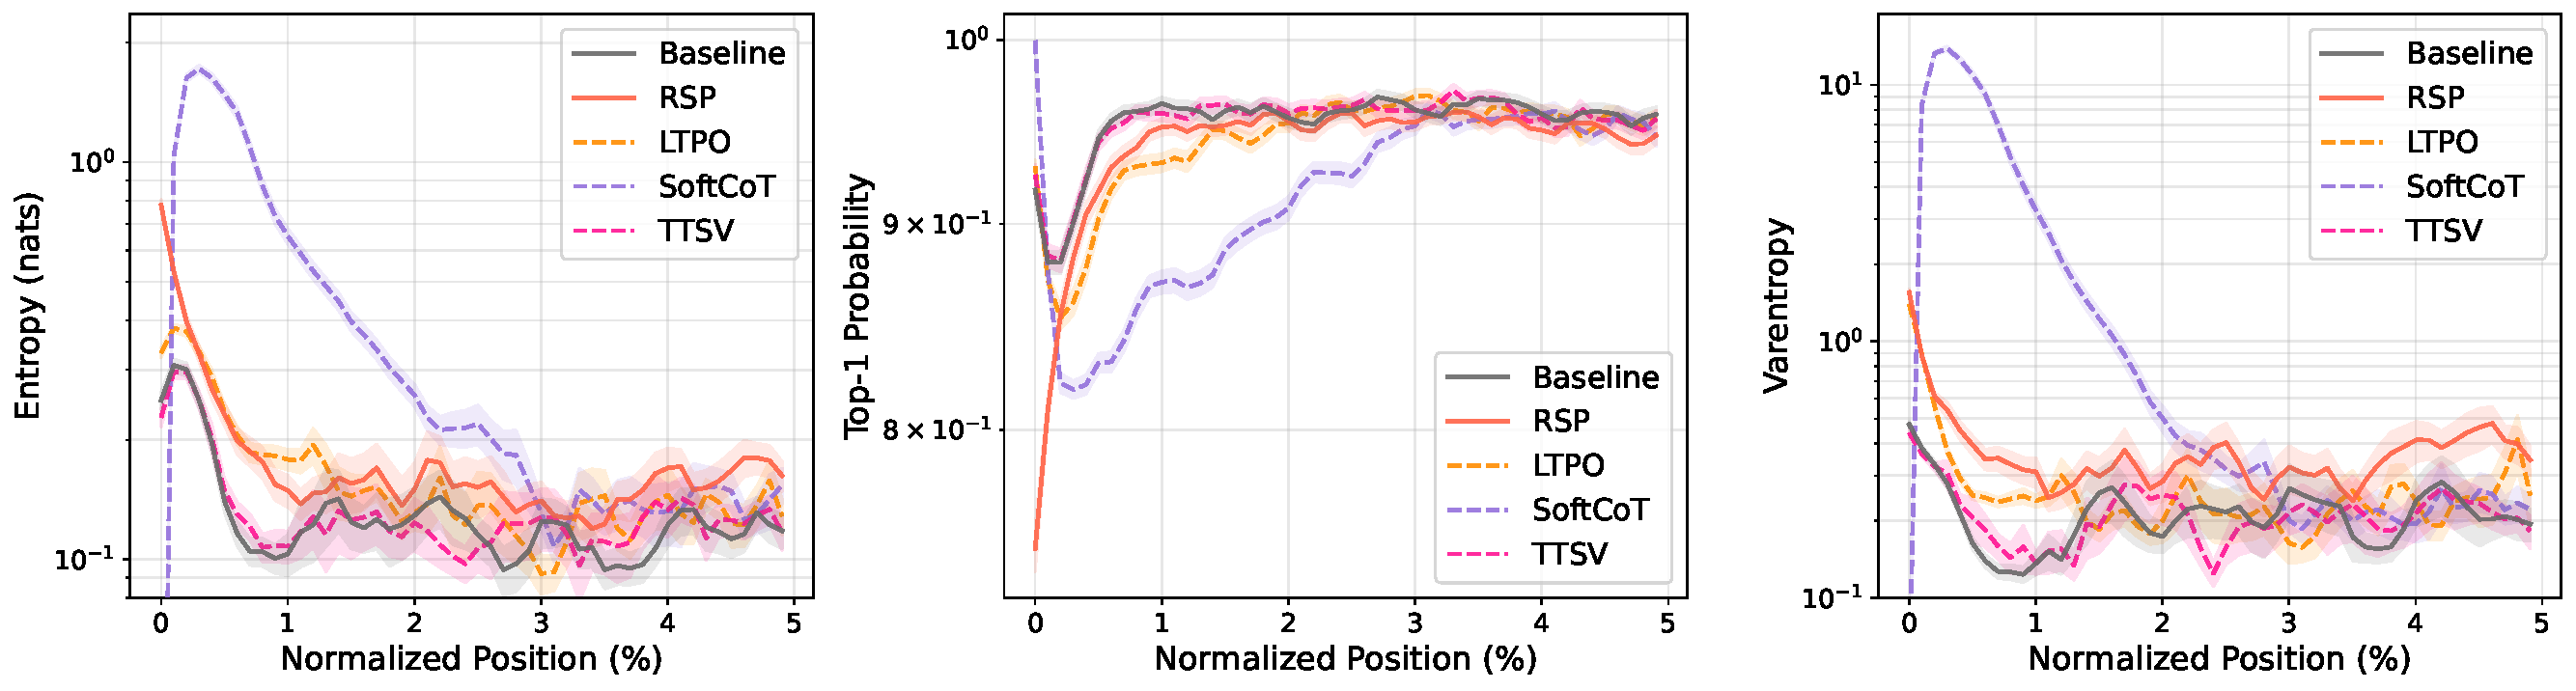
\includegraphics[width=\textwidth]{img/entropy/entropy_first5pct_zoom.pdf}
  \caption{생성 초반 5\% 구간의 평균 entropy, top-1 probability, varentropy (Qwen2.5-Math-1.5B-Instruct, MATH-500). 음영은 $\pm$1 SEM이다. 실선은 RSP 변형과 baseline, 점선은 기존 soft prompt 방법(LTPO, SoftCoT, TTSV)이다.}
  \label{fig:entropy_first5}
\end{figure}

RSP를 포함한 latent prompt 방법들은 공통적으로 \emph{생성 초반 entropy 상승 → 후반 baseline 수렴}이라는 동일한 시그니처를 보인다. 메커니즘 측면에서 자연스러운 설명은 OOV(out-of-vocabulary) 효과다 --- 어휘 바깥의 연속 임베딩이 입력으로 들어오면 모델은 익숙한 토큰 분포 위에서 한 번도 본 적 없는 키 위치를 attend해야 하므로 초반 next-token 분포에서 확률 질량이 여러 후보로 재분배된다. 세 RSP 주입 위치 모두에서 초반 entropy↑, top-1 probability↓, varentropy↑가 함께 나타나며, 이는 multimodal 분포와 정합한다 \citep{ahmed2026logitscope}. 변화가 생성 초반에 국한되고 중·후반에는 세 지표 모두 baseline 수준으로 수렴한다는 점이 중요한데, 이는 \S\ref{sec:converge}의 cache-growth attenuation이 예측한 \emph{초반 영향력 → 캐시 성장에 따른 자동 감쇠} 패턴과 정합한다.

서로 다른 목적 함수로 학습된 prior 방법(LTPO, SoftCoT, TTSV)도 같은 시그니처를 공유한다. 평균 entropy를 \emph{줄이는} 보상을 쓰는 TTSV조차 초반 구간만큼은 baseline과 비슷하다. entropy 수치 자체가 quality score가 아닌 점은 짚어 둘 만하다 --- 높은 entropy가 무조건 좋은 것이 아니라, 시그니처가 드러내는 것은 학습 목적과 무관하게 OOV 임베딩 주입이 같은 fingerprint를 만든다는 \emph{공유 메커니즘}이다. latent reasoning을 가능케 하는 핵심 요소가 학습된 의미가 아니라 \emph{주입 자체}에 있다는 가설을 이 시그니처가 뒷받침한다.

% ================================================================
\subsection{RSP는 실제로 추론 궤적의 다양성을 만드는가?}\label{sec:diversity}
% ================================================================

\S\ref{sec:entropy}는 RSP가 생성 초반 출력 분포를 바꾼다는 사실을 보였다. 이제 이 변화가 실제 추론 다양성으로 이어지는지를 세 수준에서 살펴본다. 분석 수준은 토큰 순위, 궤적의 의미적 내용, 과제 수준 결과다. 세 분석 모두 Qwen2.5-Math-1.5B-Instruct, MATH-500, \emph{suffix} 주입, $L=10$ 설정을 공유한다.

\paragraph{토큰 수준: temperature를 넘어서는 분포 변화.}
\begin{wraptable}{r}{0.55\textwidth}
  \vspace{-1.2em}
  \centering
  \caption{Baseline $\tau{=}1.0$을 기준으로 본 첫 토큰 분포 지표. 더 높은 temperature의 baseline($\tau{=}2.0,3.0$)과 RSP $\tau{=}1.0$을 비교한다. RSP 지표는 16개 random seed 평균이며, Acc는 문제당 16개 샘플의 평균 $\pm$ 표준편차다.}
  \label{tab:rsp_vs_temp}
  \footnotesize
  \setlength{\tabcolsep}{3.5pt}
  \renewcommand{\arraystretch}{0.9}
  \begin{tabular}{lccc}
    \toprule
    \textbf{Metric} & \textbf{$\tau{=}2.0$} & \textbf{$\tau{=}3.0$} & \cellcolor{blue!10}\textbf{RSP} \\
    \midrule
    Spearman $\rho$ & 1.000 & 1.000 & \cellcolor{blue!10}\textbf{0.709} \\
    Mass outside top-10 & 5.18\% & 29.11\% & \cellcolor{blue!10}\textbf{21.86\%} \\
    JS divergence & 0.060 & 0.218 & \cellcolor{blue!10}\textbf{0.131} \\
    Acc (\%) & 20.77 $\pm$ 1.47 & 1.42 $\pm$ 0.35 & \cellcolor{blue!10}\textbf{73.30 $\pm$ 1.07} \\
    \bottomrule
  \end{tabular}
\end{wraptable}
RSP가 첫 토큰 분포를 얼마나 흔드는지를 정량화한다 --- 추론 궤적의 분기점이다 \citep{wang2025beyond}. Baseline $\tau{=}1.0$을 기준으로, 더 높은 temperature($\tau{=}2.0,3.0$, 문제당 16개 샘플)과 RSP $\tau{=}1.0$(16 seed 평균)을 세 지표로 비교한다: 순위 재배치를 감지하는 Spearman rank correlation $\rho$, support 확장을 측정하는 baseline top-10 밖 확률 질량, 전체 분포 변화 크기를 정량화하는 Jensen--Shannon divergence (정식 정의는 Appendix~\ref{app:token_metrics}). Table~\ref{tab:rsp_vs_temp}의 대비는 명확하다. RSP의 분포 변화 크기는 $\tau{=}2.0$과 $\tau{=}3.0$ 사이지만 메커니즘이 다르다 --- temperature는 단조 변환이라 $\rho=1$이 강제되는 반면 RSP는 $\rho=0.709$로 순위를 일부 보존하면서 재배치한다. Pass@1 행이 비용을 드러낸다 --- temperature를 RSP와 같은 크기로 키우면 정확도는 1.42\%까지 무너지지만 RSP는 73.30\%를 유지한다. 따라서 RSP는 temperature와 근본적으로 다른 섭동을 만든다. 또한 RSP의 16 seed 정확도 변동성($\pm 1.07$)은 $\tau{=}2.0$ 16 샘플의 변동성($\pm 1.47$)과 비교 가능한 수준이다.

\paragraph{궤적 수준: 의미적 다양성.}
\begin{wraptable}{r}{0.34\textwidth}
  \vspace{-1.2em}
  \centering
  \caption{64개 문제에 대해 평균한 의미적 다양성 지표.}
  \label{tab:semantic_metrics}
  \footnotesize
  \setlength{\tabcolsep}{4pt}
  \renewcommand{\arraystretch}{0.9}
  \begin{tabular}{lcc}
    \toprule
    \textbf{Metric} & \textbf{Baseline} & \cellcolor{blue!10}\textbf{RSP} \\
    \midrule
    Pairwise cos.\ dist. & 0.0612 & \cellcolor{blue!10}\textbf{0.0879} \\
    Inter-cluster dist. & 0.0183 & \cellcolor{blue!10}\textbf{0.0982} \\
    Intra-cluster dist. & 0.0526 & \cellcolor{blue!10}0.0528 \\
    \bottomrule
  \end{tabular}
\end{wraptable}
토큰 수준 재배치는 두 번째 질문을 만든다 --- 첫 토큰 섭동이 서로 \emph{다른} 궤적으로 갈라지는가, 아니면 비슷한 궤적으로 수렴하는가? MATH-500에서 무작위 64개 문제를 뽑고, Baseline과 RSP 두 조건에서 각 문제마다 $\tau{=}1.0$으로 300개의 독립 궤적을 생성했다. 각 궤적을 BGE-M3 \citep{chen2024bge}로 임베딩하고 세 지표를 계산한다 --- 의미적 spread 전체를 보는 \textit{pairwise cosine distance}, density 기반 클러스터링 알고리즘인 DBSCAN \citep{ester1996density} 군집 중심 사이의 \textit{inter-cluster distance}(서로 다른 궤적 그룹의 분리), 그리고 군집 내 응집을 보는 \textit{intra-cluster distance}. Table~\ref{tab:semantic_metrics}는 세 패턴을 동시에 드러낸다 --- pairwise cosine distance가 1.4배로 커지고, inter-cluster distance가 5.4배로 뛰며, intra-cluster distance는 거의 변하지 않는다. 즉 궤적 집합이 더 다양해지고 더 분리된 군집들로 갈라지면서도 군집 내부 응집은 유지된다. RSP는 pairwise distance 기준으로도 64개 중 56개 문제에서 baseline보다 컸다.

\paragraph{결과 수준: Pass@$N$ 스케일링.}
마지막 결과 수준에서는, 이러한 다양성이 실제 과제 성과로 이어지는지를 Pass@$N$ \citep{chen2021codex}로 본다($N$개 샘플 중 적어도 하나가 정답일 확률). MATH-500과 AIME24에서 문제당 16개 샘플을 생성하고 네 조건을 비교한다 --- \textit{(i)} \textit{Baseline} + $\tau{=}1.0$, \textit{(ii)} \textit{RSP (single seed)} + $\tau{=}1.0$, 모든 샘플이 같은 RSP 공유, \textit{(iii)} \textit{RSP (indep.\ seed)} + greedy, 샘플마다 새 RSP, \textit{(iv)} \textit{RSP (indep.\ seed)} + $\tau{=}1.0$, 샘플마다 새 RSP.

\begin{figure}[ht]
  \centering
  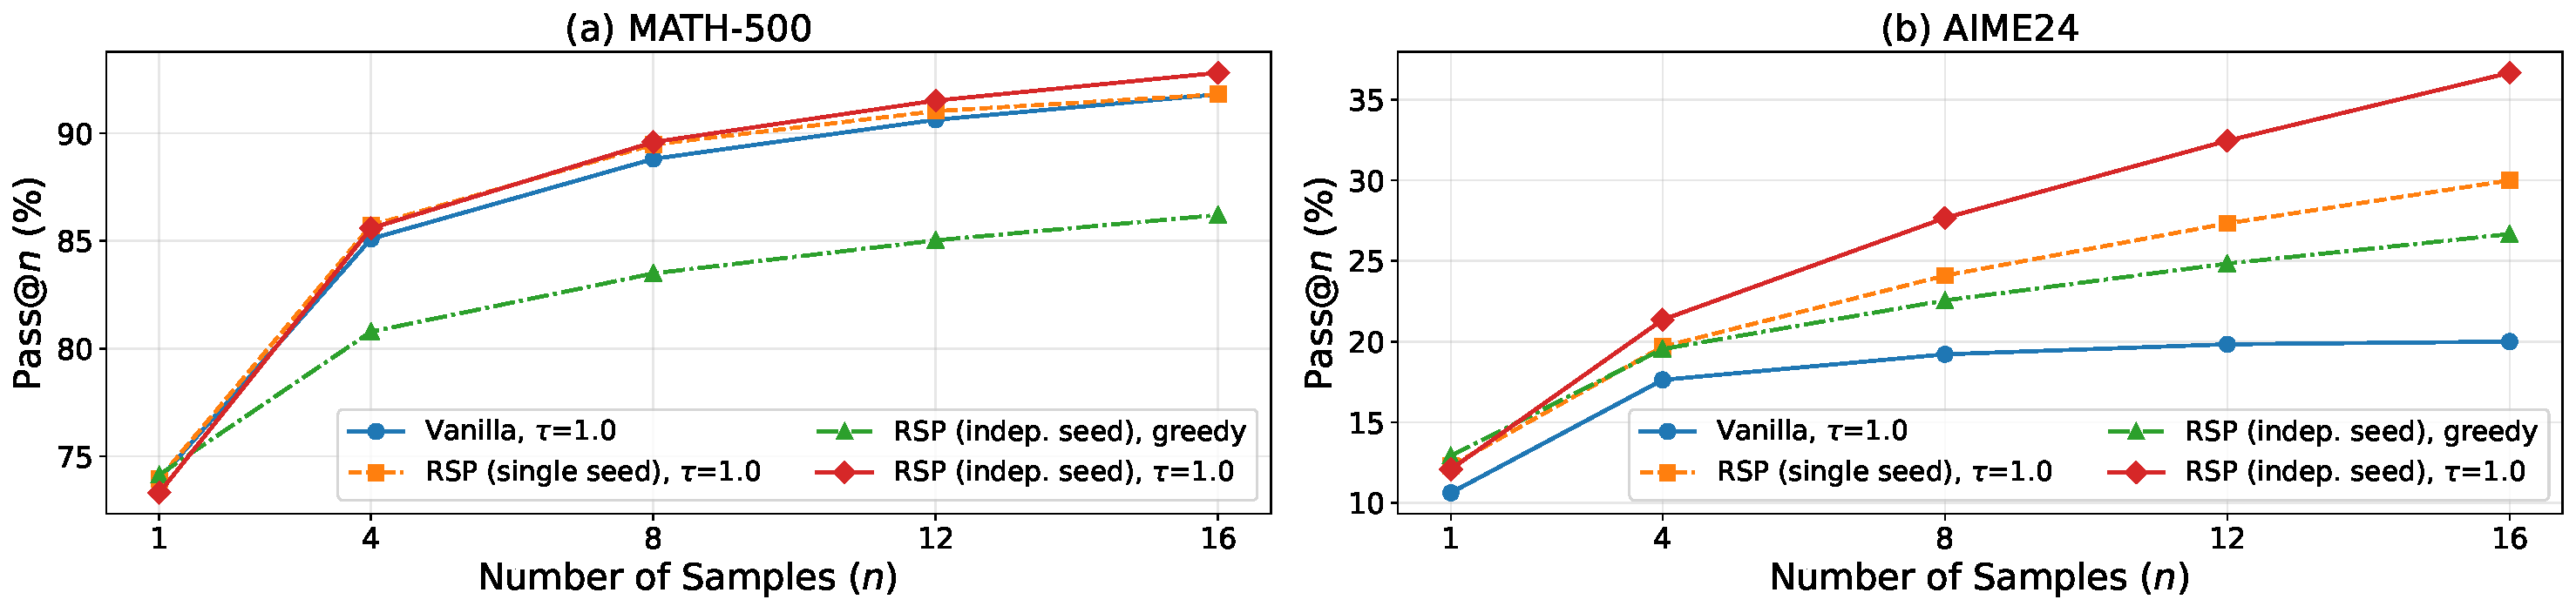
\includegraphics[width=0.9\textwidth]{img/diversity/pass_at_n_combined.pdf}
  \caption{Qwen2.5-Math-1.5B-Instruct에서의 Pass@$N$ 스케일링. 좌측은 MATH-500, 우측은 AIME24이며, 문제당 16개 샘플 사용. \textit{Baseline}: temperature sampling만. \textit{RSP (single seed)}: 고정된 하나의 RSP와 temperature를 함께. \textit{RSP (indep.\ seed)}: 샘플마다 다른 RSP를 쓰는 경우(temperature 유무).}
  \label{fig:pass_at_n}
\end{figure}

조건 \textit{(iv)}가 두 벤치마크 모두에서 가장 높은 Pass@$N$을 달성하며 $N=16$에서 MATH-500 92.80\%, AIME24 36.67\%에 이른다. \textit{(ii)}는 baseline 대비 거의 개선이 없어, 다양성 이득의 핵심이 \emph{고정} 섭동이 아니라 샘플마다 \emph{독립}된 무작위 임베딩임을 드러낸다. Pass@1은 MATH-500에서 baseline 수준을 유지하고 더 어려운 AIME24에서는 \textit{(iv)}가 더 높아, 독립 RSP + temperature 결합이 단일 샘플 정확도를 해치지 않으면서 추론 궤적을 다양화한다.
